\documentclass[11pt]{article}

%** Package ****************************************************************************************

%**** Page settings ******************************

\usepackage[%
paper=a4paper,%
landscape,
%includeheadfoot,%
margin=1cm,%
headsep=0cm, footskip=0cm,%
dvips,%
]{geometry}

%**** Encoding ***********************************

\usepackage[utf8]{inputenc}

%*************************************************

\usepackage{tikz}
\usetikzlibrary{calc} 
\usepgflibrary{arrows}
\usetikzlibrary{external}
\tikzexternalize[prefix=images/]

\usepackage{calc}

%***************************************************************************************************

% \tikzset{
%   % Defines a custom style which generates BOTH, .pdf and .png export but prefers the .png on inclusion.
%   % 
%   % This style is not pre-defined, you may need to copy-paste and adjust it.
%   png export/.style={
%     external/system call/.add=
%       {}
%       {; convert -density 300 -transparent white "\image.pdf" "\image.png"},
%     % 
%     /pgf/images/external info,
%     /pgf/images/include external/.code={%
%       \includegraphics[width=\pgfexternalwidth,height=\pgfexternalheight]{##1.png}%
%     },
%   }
% }
% \tikzset{png export}

%***************************************************************************************************

\def\Radius{40}
\def\NacelleRadius{7}
\def\ArmLength{55}
%\def\Rho{\Radius-\NacelleRadius}
\def\Rho{33}
\def\AxesLength{1.15*\Radius}

% x1 = 10, z = 10
% z1 = z + sqrt(L**2 - (x-rho)**2)
% 10 + math.sqrt(55**2 - (10-(40-7))**2)
\def\Nx{10}
\def\Nz{10}
\def\z1{59.96}
\def\AxesLengthZ{1.25*\z1}

\begin{document}
%
\pagestyle{empty}
%
\begin{center}
\tikzsetnextfilename{schema-top-view}
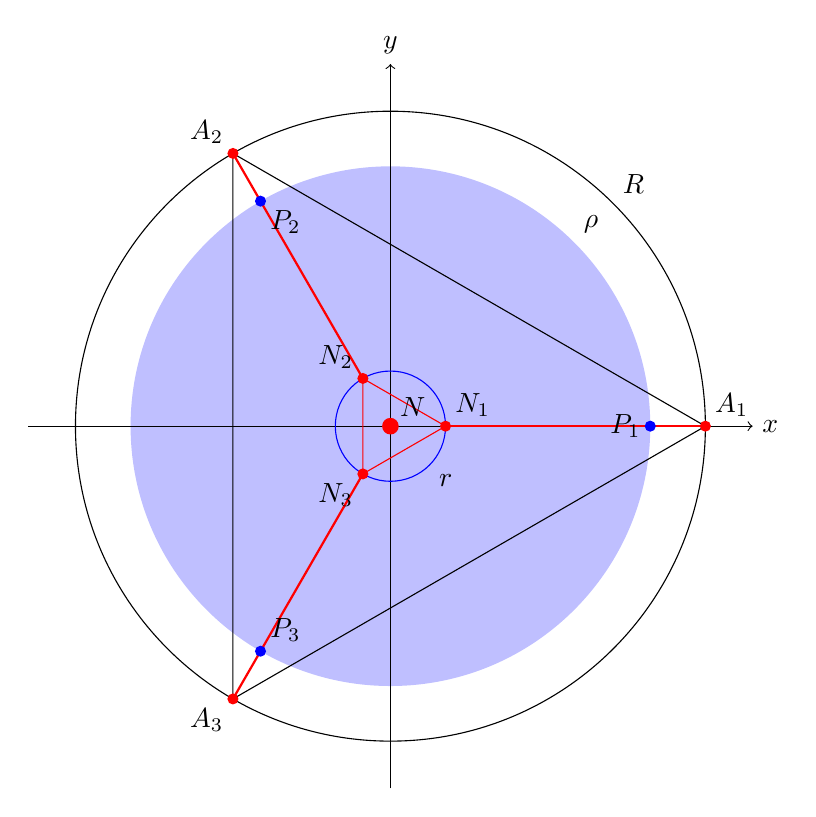
\begin{tikzpicture}[x=1mm,y=1mm]
  \coordinate (O) at (0,0);
  \coordinate (N) at (0,0);
  \coordinate (N1) at ($ (N) + (xyz polar cs:angle=0,radius=\NacelleRadius) $);
  \coordinate (N2) at ($ (N) + (xyz polar cs:angle=120,radius=\NacelleRadius) $);
  \coordinate (N3) at ($ (N) + (xyz polar cs:angle=240,radius=\NacelleRadius) $);
  \coordinate (P1) at (xyz polar cs:angle=0,radius=\Rho);
  \coordinate (P2) at (xyz polar cs:angle=120,radius=\Rho);
  \coordinate (P3) at (xyz polar cs:angle=240,radius=\Rho);
  \coordinate (A1) at (xyz polar cs:angle=0,radius=\Radius);
  \coordinate (A2) at (xyz polar cs:angle=120,radius=\Radius);
  \coordinate (A3) at (xyz polar cs:angle=240,radius=\Radius);
  % inner space
  \fill [blue!25] (O) circle(\Rho);
  % axes
  \draw[->] (-\AxesLength,0) -- (\AxesLength,0) node[right] {$x$};
  \draw[->] (0,-\AxesLength) -- (0,\AxesLength) node[above] {$y$};
  %
  \draw (O) circle(\Radius);
  \draw (A1) -- (A2) -- (A3) -- cycle;
  % nacelle
  \draw [blue] (N) circle(\NacelleRadius);
  \draw [red] (N1) -- (N2) -- (N3) -- cycle;
  %
  \foreach \point in {1,2,3}
    {
      % arms
      \draw [red, thick] (N\point) -- (A\point);
      % points
      \fill [red] (N\point) circle (2pt);
      \fill [blue] (P\point) circle (2pt);
      \fill [red] (A\point) circle (2pt);
    }
  % labels
  % \draw (O) node[anchor=south west] {$O$};
  \fill [red] (N) circle (3pt);
  \draw (N) node[anchor=south west] {$N$};
  \draw (N1) node[anchor=south west] {$N_1$};
  \draw (N2) node[anchor=south east] {$N_2$};
  \draw (N3) node[anchor=north east] {$N_3$};
  \draw (P1) node[anchor=east] {$P_1$};
  \draw (P2) node[anchor=north west] {$P_2$};
  \draw (P3) node[anchor=south west] {$P_3$};
  \draw (A1) node[anchor=south west] {$A_1$};
  \draw (A2) node[anchor=south east] {$A_2$};
  \draw (A3) node[anchor=north east] {$A_3$};
  % lengths
  % \draw ($(O)!.5!(A1)$) node[anchor=south] {$R$};
  % \draw ($(N)!.5!(-\NacelleRadius,0)$) node[anchor=south] {$r$};
  \draw (-45:\NacelleRadius) node[anchor=north west] {$r$};
  \draw (45:\Rho) node[anchor=south west] {$\rho$};
  \draw (45:\Radius) node[anchor=south west] {$R$};
\end{tikzpicture}
\end{center}
%
\begin{center}
\tikzsetnextfilename{schema-side-view}
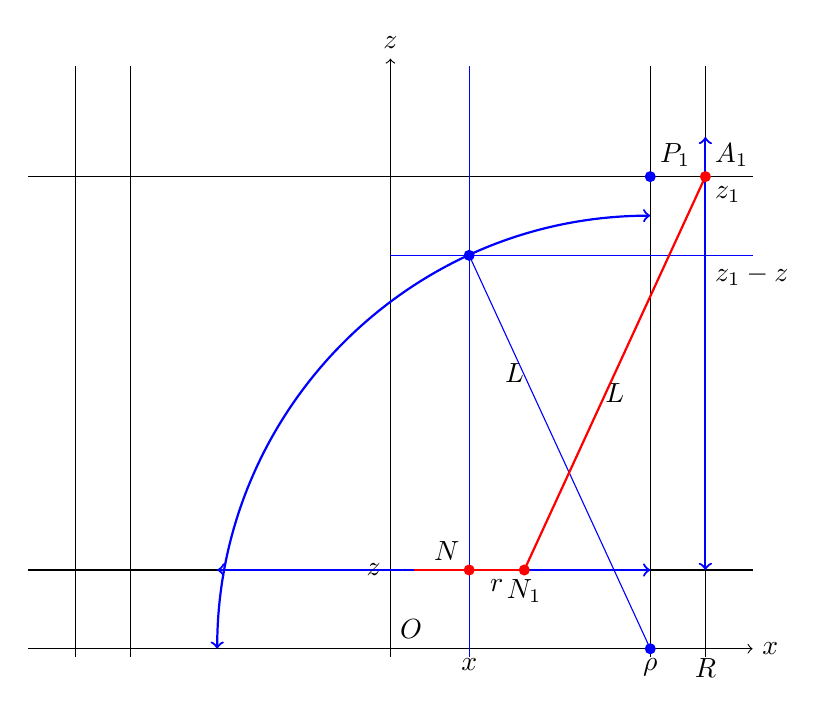
\begin{tikzpicture}[x=1mm,y=1mm]
  \coordinate (O) at (0,0);
  \coordinate (N) at (\Nx,\Nz);
  \coordinate (N1) at ($ (N) + (\NacelleRadius,0) $);
  \coordinate (A1) at (\Radius,\z1);
  \coordinate (P1) at (\Rho,\z1);
  % axes
  \draw[->] (-\AxesLength,0) -- (\AxesLength,0) node[right] {$x$};
  \draw[->] (0,-1) -- (0,\AxesLengthZ) node[above] {$z$};
  \draw (-\AxesLength,\Nz) -- (\AxesLength,\Nz);
  \draw (-\AxesLength,\z1) -- (\AxesLength,\z1);
  \draw (\Radius,-1) -- +(0,\AxesLengthZ);
  \draw (-\Radius,-1) -- +(0,\AxesLengthZ);
  \draw (\Rho,-1) -- +(0,\AxesLengthZ);
  \draw (-\Rho,-1) -- +(0,\AxesLengthZ);
  % z curve
  \coordinate (C) at (\Rho,0);
  \coordinate (Pcx) at (\Nx,-1);
  \coordinate (Pcy) at (0,\z1-\Nz);
  \coordinate (Pc) at (\Nx,\z1-\Nz);
  \begin{scope}[blue, fill=blue]
    \draw (Pcx) -- +(0,\AxesLengthZ);
    \draw (Pcy) -- +(\AxesLength,0);
    \fill (Pc) circle (2pt);
    \draw (C) -- (Pc);
    \draw [<->, thick] (\Radius,\Nz) -- +(0,\ArmLength);
    \draw [<->, thick] (\Rho,\Nz) -- +(-\ArmLength,0);
    % \fill (\Rho,\Nz) circle (2pt);
    % \clip (-\Rho,0) rectangle(\Rho,\ArmLength);
    % \draw (C) circle(\ArmLength);
    \draw[<->, thick] (\Rho, \ArmLength) arc [start angle=90, end angle=180, x radius=\ArmLength, y radius=\ArmLength];
  \end{scope}
  % nacelle
  \draw [red, thick] ($ (N) - (\NacelleRadius,0) $) -- (N1);
  % arm
  \draw [red, thick] (N1) -- (A1);
  % labels
  \draw (O) node[anchor=south west] {$O$};
  \draw (N) node[anchor=south east] {$N$};
  \draw (N1) node[anchor=north] {$N_1$};
  \draw (A1) node[anchor=south west] {$A_1$};
  \draw (P1) node[anchor=south west] {$P_1$};
  \fill [red] (N) circle (2pt);
  \fill [red] (N1) circle (2pt);
  \fill [red] (A1) circle (2pt);
  \fill [blue] (P1) circle (2pt);
  \fill [blue] (\Rho,0) circle (2pt); % z curve center
  % lengths
  % \draw ($(O)!.5!(\Radius,0)$) node[anchor=south] {$R$};
  \draw (\Radius,0) node[anchor=north] {$R$};
  \draw (\Rho,0) node[anchor=north] {$\rho$};
  % \draw ($(\Radius,0)!.5!(A1)$) node[anchor=west] {$z_1$};
  \draw (A1) node[anchor=north west] {$z_1$};
  \draw ($ (Pcy) + (\Radius,0) $) node[anchor=north west] {$z_1-z$};
  \draw (\Nx,0) node[anchor=north] {$x$};
  \draw (0,\Nz) node[anchor=east] {$z$};
  \draw ($(N1)!.5!(A1)$) node[anchor=north] {$L$};
  \draw ($(C)!.75!(Pc)$) node[anchor=north] {$L$};
  \draw ($(N)!.5!(N1)$) node[anchor=north] {$r$};
  % \draw (N1) circle(\ArmLength);
  % \draw (A1) circle(\ArmLength);
  % \draw (P1) circle(\ArmLength);
\end{tikzpicture}
\end{center}
%
\begin{center}
\tikzsetnextfilename{schema-top-view-moved}
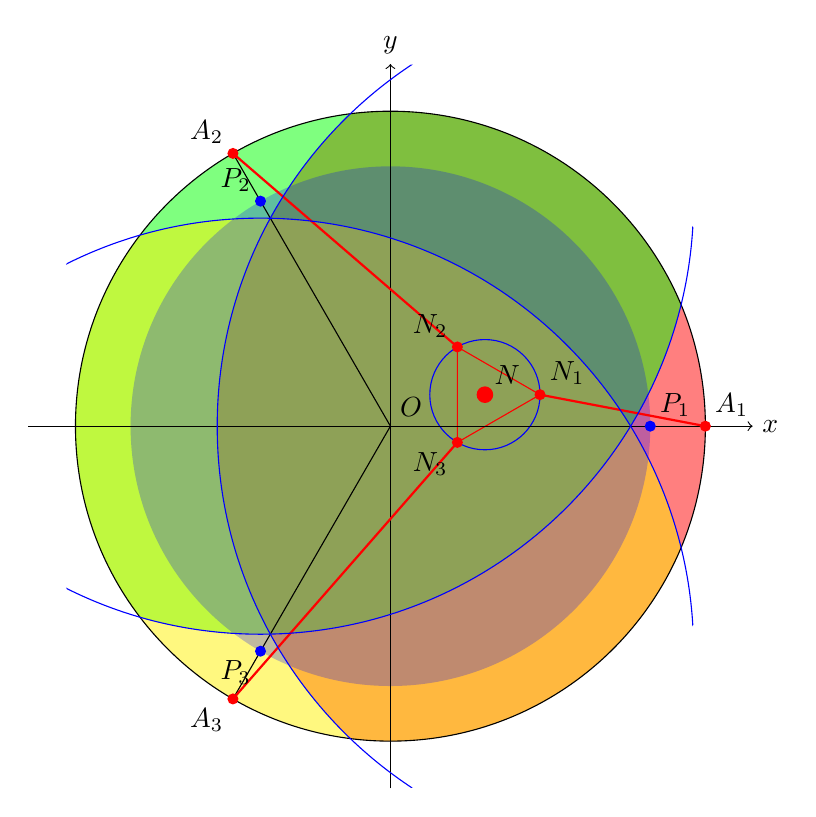
\begin{tikzpicture}[x=1mm,y=1mm]
  \coordinate (O) at (0,0);
  \coordinate (N) at (.3*\Radius,.1*\Radius);
  \coordinate (N1) at ($ (N) + (xyz polar cs:angle=0,radius=\NacelleRadius) $);
  \coordinate (N2) at ($ (N) + (xyz polar cs:angle=120,radius=\NacelleRadius) $);
  \coordinate (N3) at ($ (N) + (xyz polar cs:angle=240,radius=\NacelleRadius) $);
  \coordinate (P1) at (xyz polar cs:angle=0,radius=\Rho);
  \coordinate (P2) at (xyz polar cs:angle=120,radius=\Rho);
  \coordinate (P3) at (xyz polar cs:angle=240,radius=\Rho);
  \coordinate (A1) at (xyz polar cs:angle=0,radius=\Radius);
  \coordinate (A2) at (xyz polar cs:angle=120,radius=\Radius);
  \coordinate (A3) at (xyz polar cs:angle=240,radius=\Radius);
  % working space
  \begin{scope}[fill=red, fill opacity=.5]
    \clip (O) circle(\Radius);
    \fill (P1) circle(\ArmLength);
  \end{scope}
  \begin{scope}[fill=green, fill opacity=.5]
    \clip (O) circle(\Radius);
    \fill (P2) circle(\ArmLength);
  \end{scope}
  \begin{scope}[fill=yellow, fill opacity=.5]
    \clip (O) circle(\Radius);
    \fill (P3) circle(\ArmLength);
  \end{scope}
  % inner space
  \fill [blue, fill opacity=.25] (O) circle(\Rho);
  % axes
  \draw[->] (-\AxesLength,0) -- (\AxesLength,0) node[right] {$x$};
  \draw[->] (0,-\AxesLength) -- (0,\AxesLength) node[above] {$y$};
  %
  \draw (O) circle(\Radius);
  \draw [blue] (N) circle(\NacelleRadius);
  % \draw (A1) -- (A2) -- (A3) -- cycle;
  % nacelle
  \draw [red] (N1) -- (N2) -- (N3) -- cycle;
  % 
  \foreach \point in {1,2,3}
    {
      \draw (O) -- (A\point);
      % arms
      \draw [red, thick] (N\point) -- (A\point);
      % \draw [blue] (P\point) circle(\ArmLength);
      % points
      \fill [red] (N\point) circle (2pt);
      \fill [blue] (P\point) circle (2pt);
      \fill [red] (A\point) circle (2pt);
    }
  \begin{scope}
    \clip (O) circle(\AxesLength);
    \foreach \point in {1,2,3}
    {
      \draw [blue] (P\point) circle(\ArmLength);
    }
  \end{scope}
  % labels
  \fill [red] (N) circle (3pt);
  \draw (O) node[anchor=south west] {$O$};
  \draw (N) node[anchor=south west] {$N$};
  \draw (N1) node[anchor=south west] {$N_1$};
  \draw (N2) node[anchor=south east] {$N_2$};
  \draw (N3) node[anchor=north east] {$N_3$};
  \draw (P1) node[anchor=south west] {$P_1$};
  \draw (P2) node[anchor=south east] {$P_2$};
  \draw (P3) node[anchor=north east] {$P_3$};
  \draw (A1) node[anchor=south west] {$A_1$};
  \draw (A2) node[anchor=south east] {$A_2$};
  \draw (A3) node[anchor=north east] {$A_3$};
 \end{tikzpicture}
\end{center}
%
%
\begin{center}
\tikzsetnextfilename{schema-top-view-moved-sphere}
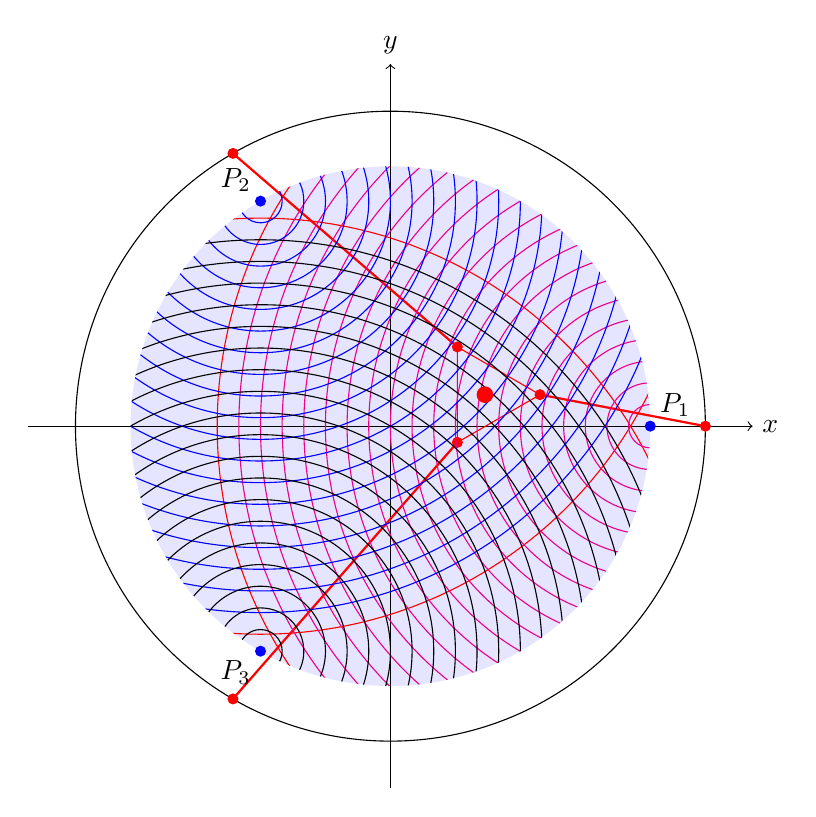
\begin{tikzpicture}[x=1mm,y=1mm]
  \coordinate (O) at (0,0);
  \coordinate (N) at (.3*\Radius,.1*\Radius);
  \coordinate (N1) at ($ (N) + (xyz polar cs:angle=0,radius=\NacelleRadius) $);
  \coordinate (N2) at ($ (N) + (xyz polar cs:angle=120,radius=\NacelleRadius) $);
  \coordinate (N3) at ($ (N) + (xyz polar cs:angle=240,radius=\NacelleRadius) $);
  \coordinate (P1) at (xyz polar cs:angle=0,radius=\Rho);
  \coordinate (P2) at (xyz polar cs:angle=120,radius=\Rho);
  \coordinate (P3) at (xyz polar cs:angle=240,radius=\Rho);
  \coordinate (A1) at (xyz polar cs:angle=0,radius=\Radius);
  \coordinate (A2) at (xyz polar cs:angle=120,radius=\Radius);
  \coordinate (A3) at (xyz polar cs:angle=240,radius=\Radius);
  % working space
  % \begin{scope}[fill=red, fill opacity=.5]
  %   \clip (O) circle(\Radius);
  %   \fill (P1) circle(\ArmLength);
  % \end{scope}
  % \begin{scope}[fill=green, fill opacity=.5]
  %   \clip (O) circle(\Radius);
  %   \fill (P2) circle(\ArmLength);
  % \end{scope}
  % \begin{scope}[fill=yellow, fill opacity=.5]
  %   \clip (O) circle(\Radius);
  %   \fill (P3) circle(\ArmLength);
  % \end{scope}
  % inner space
  \fill [blue, fill opacity=.10] (O) circle(\Rho);
  % \draw [blue] (O) circle(\Rho);
  % axes
  \draw[->] (-\AxesLength,0) -- (\AxesLength,0) node[right] {$x$};
  \draw[->] (0,-\AxesLength) -- (0,\AxesLength) node[above] {$y$};
  %
  \draw (O) circle(\Radius);
  % \draw [blue] (N) circle(\NacelleRadius);
  % \draw (A1) -- (A2) -- (A3) -- cycle;
  \draw [red] (N1) -- (N2) -- (N3) -- cycle;
  % 
  \foreach \point in {1,2,3}
    {
      % \draw (O) -- (A\point);
      % arms
      \draw [red, thick] (N\point) -- (A\point);
      % \draw [blue] (P\point) circle(\ArmLength);
      % points
      \fill [red] (N\point) circle (2pt);
      \fill [blue] (P\point) circle (2pt);
      \fill [red] (A\point) circle (2pt);
    }
  \begin{scope}
    \clip (O) circle(\Rho);
    \foreach \point in {1,2,3}
    {
      \draw [red] (P\point) circle(\ArmLength);
    }
    \foreach \i in {.05,.1,...,1.}
    {
      \draw [magenta] (P1) circle(\i*\ArmLength);
    }
    \foreach \i in {.05,.1,...,1.}
    {
      \draw [blue] (P2) circle(\i*\ArmLength);
    }
    \foreach \i in {.05,.1,...,1.}
    {
      \draw [black] (P3) circle(\i*\ArmLength);
    }
  \end{scope}
    % \foreach \i in {30,40,...,90}
    % {
    %   \draw [magenta] (P1) -- +(\i+120:\ArmLength);
    %   \draw [green] (P2) -- +(\i-120:\ArmLength);
    %   \draw [yellow] (P3) -- +(\i:\ArmLength);
    % }
  % labels
  \fill [red] (N) circle (3pt);
  % \draw (O) node[anchor=south west] {$O$};
  % \draw (N) node[anchor=south west] {$N$};
  % \draw (N1) node[anchor=south west] {$N_1$};
  % \draw (N2) node[anchor=south east] {$N_2$};
  % \draw (N3) node[anchor=north east] {$N_3$};
  \draw (P1) node[anchor=south west] {$P_1$};
  \draw (P2) node[anchor=south east] {$P_2$};
  \draw (P3) node[anchor=north east] {$P_3$};
  % \draw (A1) node[anchor=south west] {$A_1$};
  % \draw (A2) node[anchor=south east] {$A_2$};
  % \draw (A3) node[anchor=north east] {$A_3$};
 \end{tikzpicture}
\end{center}
%
\end{document}

%%%%%%%%%%%%%%%%%%%%%%%%%%%%%%%%%%%%%%%%%%%%%%%%%%%%%%%%%%%%%%%%%%%%%%%%%%%%%%%%%%%%%%%%%%%%%%%%%%%%%%%%%%%%%%%%%%%%%%%%
%%%
%%% Local Variables: 
%%% mode: latex
%%% TeX-master: "master"
%%% End: 
%%%
%%%%%%%%%%%%%%%%%%%%%%%%%%%%%%%%%%%%%%%%%%%%%%%%%%%%%%%%%%%%%%%%%%%%%%%%%%%%%%%%%%%%%%%%%%%%%%%%%%%%%%%%%%%%%%%%%%%%%%%%
